\chapter{Arquiteturas \ac{mmorpg} identificadas}
\label{cap21}

Dentre as arquiteturas identificadas, as qualificadas dentro do paradigma de arquiteturas de microsserviços são as arquiteturas Rudy (Subseção~\ref{rudy}), Salz (Subseção~\ref{salz}) e Willson (Subseção~\ref{willson}).

Em geral, as arquiteturas de forma genérica contém microsserviços \textit{web} para \textit{E Commerce}, operações \ac{crud} através da web e distribuição de atualizações.
%
Os microsserviços de gerenciamento de jogo, por sua vez, respondem através do protocolo \ac{tcp}, podendo ser sobre \ac{rpc} ou protocolos proprietários.
%
A gerência de jogo é a principal mudança entre as arquiteturas, na qual contém abordagens de paralelismo diferentes:

\begin{itemize}
 \item A arquitetura Rudy (Subseção~\ref{rudy}) utiliza uma abordagem com um número menor de microsserviços, focado em manter serviços para consulta de dados de forma eficiente entre os serviços \textit{web} e o serviços de gerenciamento de jogo.
 \item A arquitetura Salz (Subseção~\ref{salz}) aborda um modelo de paralelismo mais complexo comparado a arquitetura Rudy, utilizando diversos microsserviços para funções específicas das funcionalidades do jogo.
%
Dessa forma, o ambiente do jogo torna-se escalável ao número de jogadores, porém a latência tende a aumentar.
\item A arquitetura Willson (Subseção~\ref{willson}) utiliza um modelo intermediário, evitando a divisão em múltiplos serviços para o gerente de jogo e utilizando um modelo de paralelismo próximo a arquitetura Salz.
\end{itemize}


\subsection{Arquitetura elaborada por Rudy}
\label{rudy}


A arquitetura Rudy~\cite{matthiasrudy2011} tem como objetivo criar múltiplos mundos isolados, na qual cada microsserviço será responsável por um ambiente a qual não compartilha dados com os demais ambientes.
%
Esta é uma característica importante para esta arquitetura, visto que o processamento de ações pelo serviço de jogo não precisa lidar com múltiplos processos~\cite{matthiasrudy2011}.
%
Esta arquitetura pode ser visualizada na Figura~\ref{full_rudy}.

\begin{figure}[htb!]
  \caption{Arquitetura Rudy completa.}
  \label{full_rudy}
  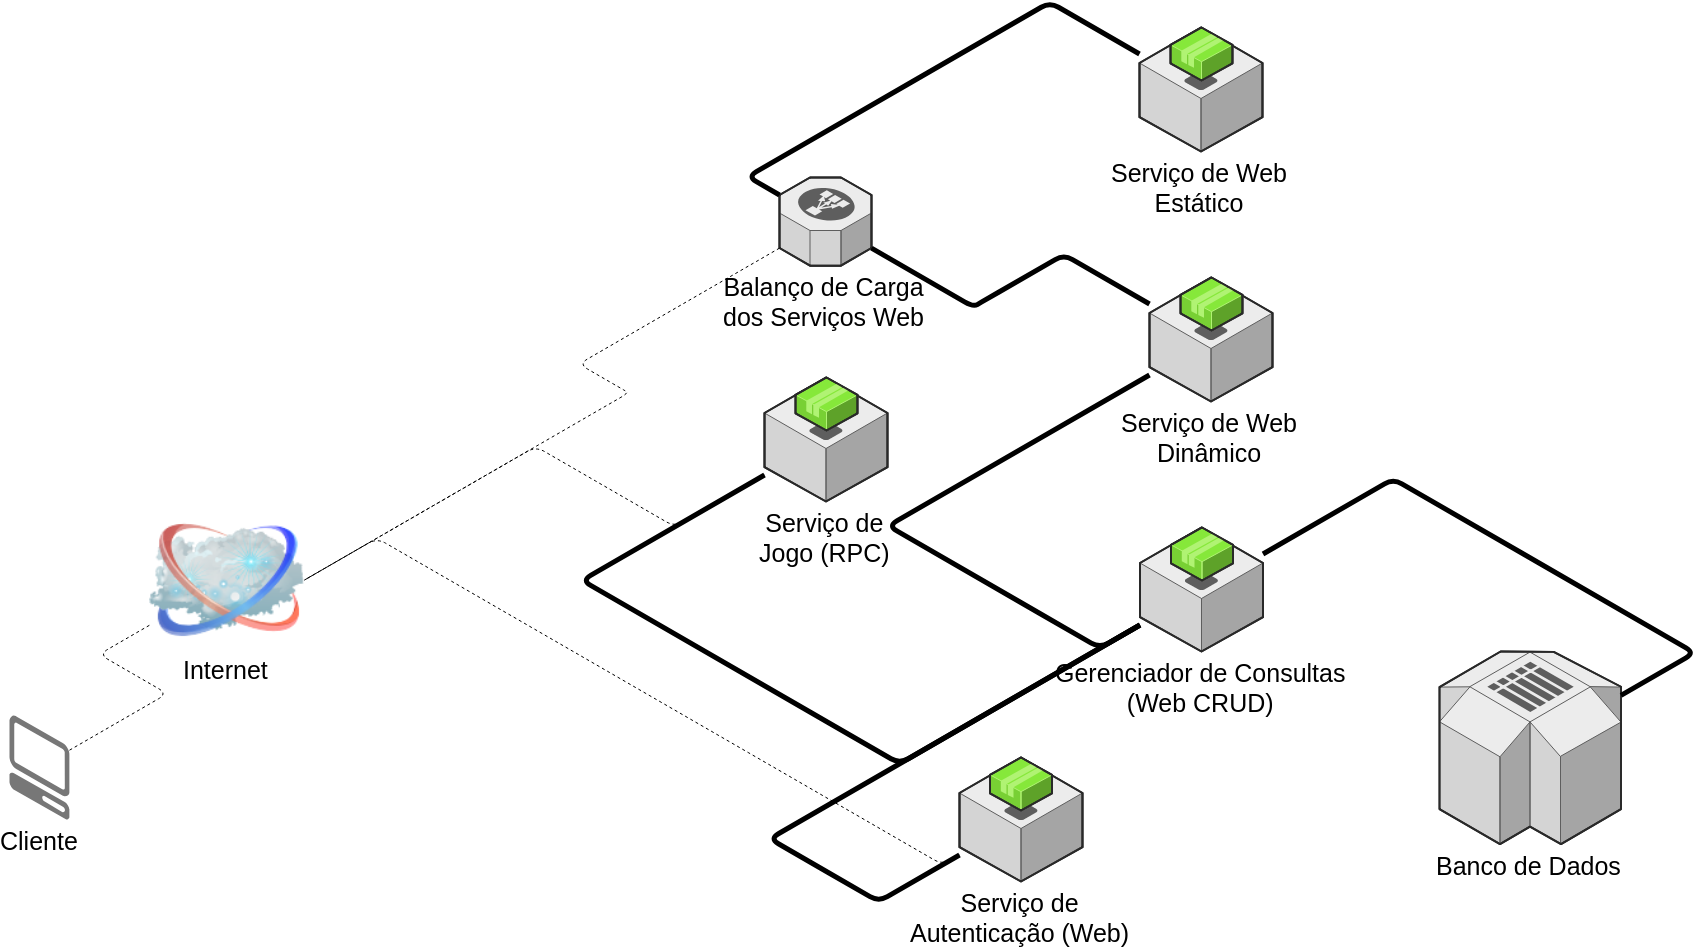
\includegraphics[width=\textwidth]{arquiteturas/full_rudy.png}
  \centering

  Adaptado de:~\cite{matthiasrudy2011}.
\end{figure}

No total, seis microsserviços distintos constam na arquitetura Rudy (Figura~\ref{full_rudy}) para o seu funcionamento, não sendo necessário o microsserviço de pagamento (utilizado somente para regra de negócios).
%
Os microsserviços que compõem a arquitetura são definidos pelas suas seguintes responsabilidades~\cite{matthiasrudy2011}:

\begin{enumerate}
  \item \textbf{Serviço de web estático}: Armazena documentos estáticos para o serviço web (\textit{e.g., }imagens, executáveis do jogo, páginas web fixas, etc). Responde sobre o protocolo \ac{http}.
  \item \textbf{Serviço de web dinâmico}: Sistema web para cadastro de contas, guias, informações sobre atualizações, compras e demais demanda de páginas dinâmicas. Responde sobre o protocolo \ac{http}.
  \item \textbf{Balanço de carga web}: Realiza a distribuição de carga sobre o \textit{Serviço web estático} e o \textit{Serviço web dinâmico}. Responde sobre o protocolo \ac{http}.
  \item \textbf{Serviço de Jogo}: Gerencia um mundo inteiro, em um único serviço. Esta abordagem segrega os jogadores em diversos canais, contendo um número máximo de conexões por canal. Cada canal opera sobre uma instância deste microsserviço. Este serviço opera sobre o protocolo \ac{rpc}.
  \item \textbf{Serviço de Autenticação}: Gerencia a autenticação das conexões ao \textit{Serviço de jogo}. Este serviço opera sobre o protocolo \ac{rpc}.
  \item \textbf{Gerenciador de Consultas}: Realiza consultas em memória e disco, utilizando vários bancos de dados diferentes, simulando o uso de banco de dados distribuídos, algo complexo de ser implementado utilizando banco de dados SQL (\textit{e.g.,} PostgreSQL\footnote{PostgreSQL: \url{https://www.postgresql.org}}, MySQL\footnote{MySQL: \url{https://www.mysql.com/}}, etc). Este serviço opera sobre o protocolo \ac{http}.
\end{enumerate}


No contexto do atual trabalho, o serviço de pagamento será ignorado, visto que ele não serve para o funcionamento básico do serviço.
%
Dentre todos os microsserviços, o usuário só tem acesso ao serviço de balanço de carga pelo protocolo \ac{http} e o serviço de jogo sobre o protocolo \ac{rpc}, tendo os demais serviços protegidos por um \textit{firewall}~\cite{matthiasrudy2011}.
%
A proteção do \textit{firewall} é aplicada no serviço de pagamento e no ponto de acesso ao serviço, podendo ser visualizada na Figura~\ref{full_rudy_fw}.


\begin{figure}[htb!]
  \caption{Arquitetura Rudy completa com \textit{firewall}.}
  \label{full_rudy_fw}
  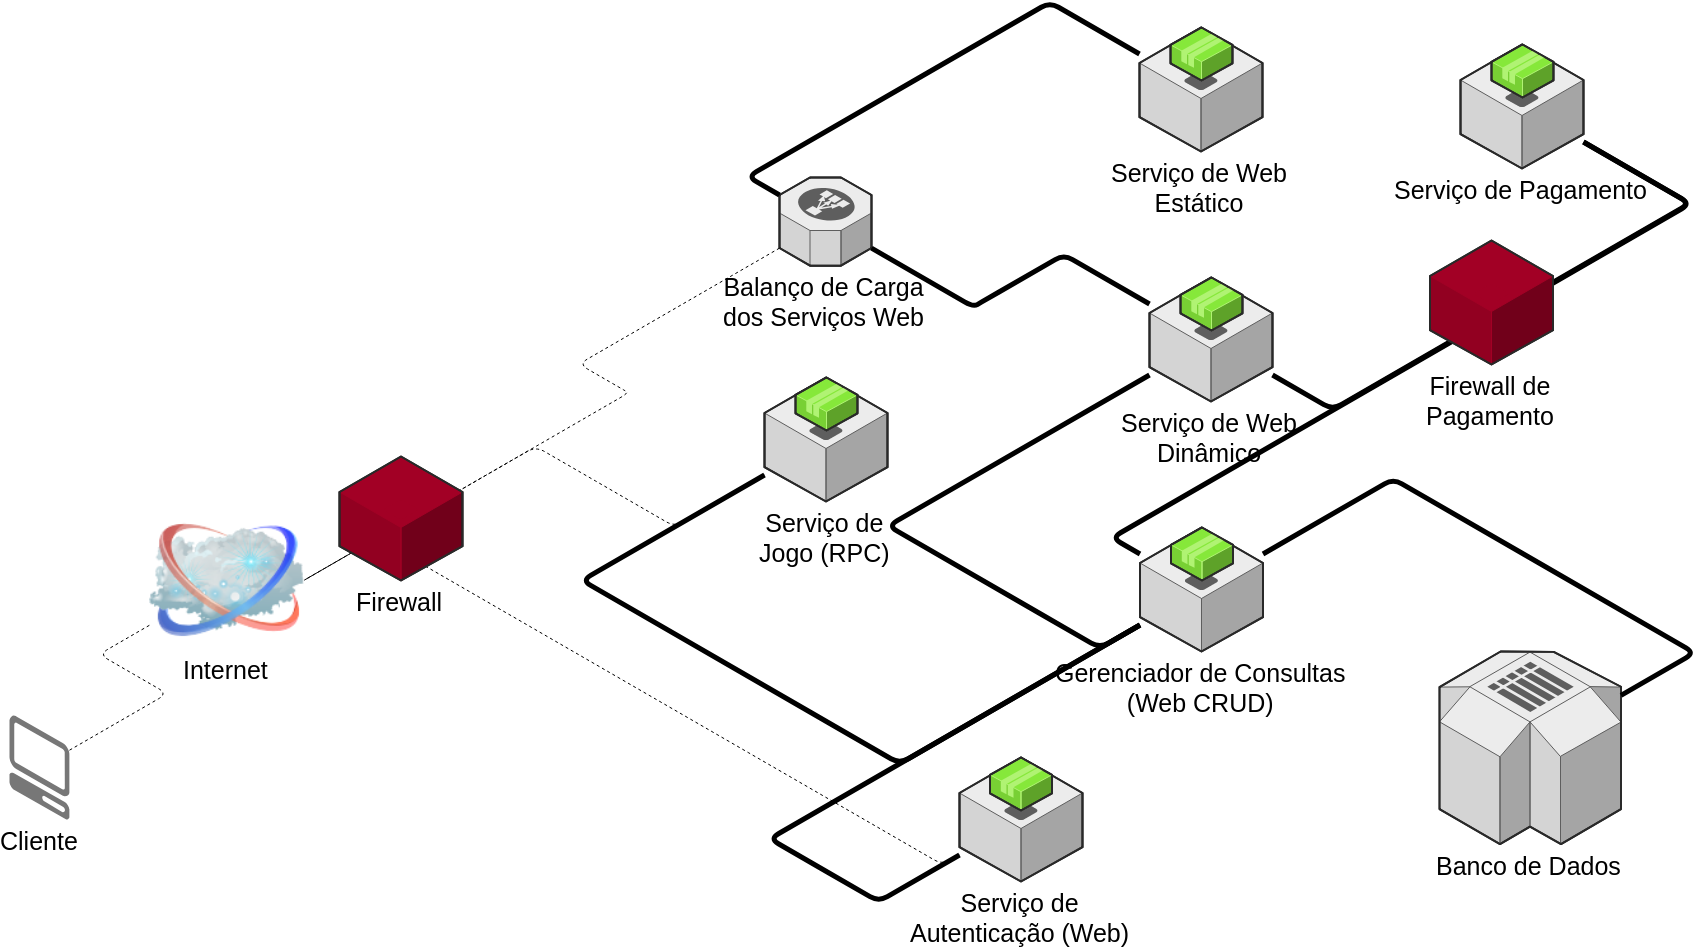
\includegraphics[width=\textwidth]{arquiteturas/full_rudy_fw.png}
  \centering

  Adaptado de:~\cite{matthiasrudy2011}.
\end{figure}




O funcionamento interno do serviço de jogo trabalha em rodadas, visando não penalizar usuários com baixa transferência de dados entre o cliente e o serviço.
%
Cada cliente produz requisições para ser consumido pelo ciclo de processamento do gerente de jogo.
%
Entretanto, o serviço irá consumir de forma igualitária uma requisição de um jogador diferente, como uma fila~\cite{albion_online_unite, matthiasrudy2011}.
%
O modelo de processamento do gerente de ambiente pode ser visualizado na Figura~\ref{fig:thread_pool}.


\begin{figure}[htb!]
  \caption{Modelo de processos \textit{Thread Pool}.}
  \label{fig:thread_pool}
  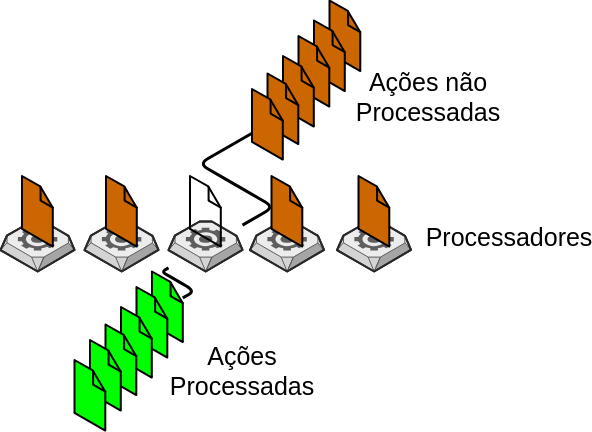
\includegraphics[height=6.5cm]{arquiteturas/thread_pool.png}
  \centering

  Adaptado de:~\cite{matthiasrudy2011, Ringler2014Dec}.
\end{figure}

O modelo de processamento do gerente de mundo, visualizado na Figura~\ref{fig:thread_pool} trabalha com um a padrão \textit{Thread Pool}~\cite{Ringler2014Dec, matthiasrudy2011}, executando a chamada de método remoto de cada jogador em uma fila, o qual prioriza executar as chamadas sem repetir a mesma conexão.
%
Dessa forma, cada jogador pode executar somente um método concorrente, sem competir com os demais. Todas as requisições são enfileiradas no \textit{buffer} de rede do serviço.
%
Caso o cliente entre em sua vez de processamento, e nenhuma chamada remota esteja na fila, ele é pulado.



Um serviço que demanda atenção na arquitetura Rudy é o Gerenciador de Consultas, um serviço web que implementa uma camada sobre diversos bancos de dados a fim de prover variedade entre vários bancos de forma facilitada por requisições web, utilizando operações \ac{crud}.
%
Implementar esta camada garante uma padronização de acesso ao banco de dados, porém adiciona um possível gargalo a arquitetura~\cite{matthiasrudy2011}.
%
Os pontos positivos de utilizar esta camada de consultas na arquitetura São:
\begin{enumerate}
  \item Não permite acesso direto ao banco de dados do serviço web e do serviço de jogo.
  \item Permite maior manejo a migrações em tabelas e troca de tecnologias.
  \item Define uma sintaxe estrita para consulta, via \ac{crud}.
  \item Permite acesso do banco a diversos serviços, sem gerenciar o banco.
  \item Permite contar número de requisições e tempo das requisições.
\end{enumerate}



Contudo, adicionando uma camada sobre os bancos de dados para gerenciamento tem pontos negativos~\cite{matthiasrudy2011}.

\begin{enumerate}
  \item Aumenta a complexidade de implementação, teste, administração e ponto de falha.
  \item Adiciona limites como número de conexões, número de requisições, etc.
\end{enumerate}

Entretanto, esta arquitetura não permite escalar um único ambiente para um número de jogadores simultâneos maior a qual o hardware que hospeda o serviço é designado.
%
Para este motivo, as arquiteturas Salz e Willson tomam abordagens para subdividir o ambiente do jogo em mais serviços, podendo assim escalar um único ambiente para mais jogadores simultâneos.


\subsection{Arquitetura elaborada por Salz}
\label{salz}

A arquitetura elaborada por Salz~\cite{albion_online_unite}, a qual pode ser visualizada na Figura~\ref{full_salz} contém sete microsserviços especializados para seu funcionamento.
%
Para o funcionamento adequado, o cliente necessita manter três conexões abertas com o servidor, sendo a conexão de jogo a com maior demanda de banda e a qual necessita o menor tempo de latência~\cite{albion_online_unite}.

\begin{figure}[htb!]
  \caption{Arquitetura Salz.}
  \label{full_salz}
  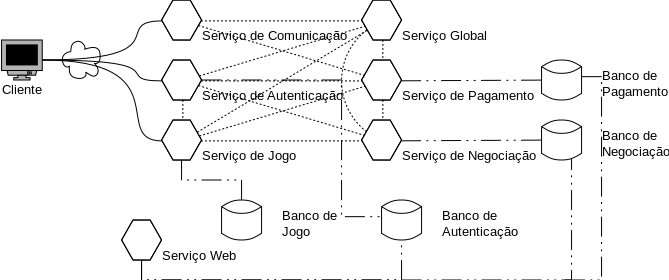
\includegraphics[width=\textwidth]{arquiteturas/full_salz.png}
  \centering

  Adaptado de:~\cite{albion_online_unite}.
\end{figure}



A Figura~\ref{full_salz} exibe a arquitetura Salz de forma completa.
%
Na Figura~\ref{full_salz} encontram-se quatro bancos de dados distintos, sendo eles o banco de \textit{Pagamento}, \textit{Negociação}, \textit{Autenticação} e \textit{Jogo}, sendo os bancos de Autenticação e Jogo com tecnologias \ac{nosql}, sendo os demais bancos com tecnologia \ac{sql}.
%
Referente aos microsserviços que compõem a arquitetura, tem-se os seguintes elementos~\cite{salz_albion}:



\begin{enumerate}
  \item \textbf{Serviço de Comunicação}: Gerencia a troca de mensagens entre os jogadores. Opera sobre o protocolo \ac{rpc}.
  \item \textbf{Serviço de Autenticação}: Recepciona e gerencia as conexões dos clientes entre os demais microsserviços. Opera sobre o protocolo \ac{http}.
  \item \textbf{Serviço de Jogo}: Gerencia o estado do mundo, referente a um \textit{chunk} do ambiente. Opera sobre o protocolo \ac{rpc}.
  \item \textbf{Serviço Global}: Gerencia operações globais (\textit{e.g,} interações entre grupos, procedimentos recorrentes globais, \textit{etc.}). Opera sobre \ac{http}.
  \item \textbf{Serviço de Pagamento}: Efetua operações bancárias com serviços externos de pagamento e gerencia o estado de pagamento das contas. Opera sobre o protocolo \ac{http}.
  \item \textbf{Serviço de Negociação}: Opera como um serviço de leilão para itens do jogo. Opera sobre o protocolo \ac{http}.
\end{enumerate}



Os microsserviços que compõem a arquitetura Salz utiliza em grande parte serviços \textit{web}, utilizando somente o protocolo \ac{rpc} para o serviço de jogo.
%
No serviço de jogo, tanto o cliente quando o serviço podem invocar métodos remotos através do protocolo \ac{rpc}, tendo como padrão métodos com retorno nulo~\cite{salz_albion, photon_serialization}.
%
Esta abordagem garante que o usuário não fique esperando pelo retorno do serviço para continuar a lógica do jogo~\cite{faber}.
%
Para este funcionamento, o modelo de processamento paralelo deste serviço possui mais regras, a qual não são abordadas pela arquitetura Rudy (Figura~\ref{full_rudy}).
%
O modelo de paralelismo do serviço de jogo pode ser visualizado na Figura~\ref{salz_thread_model}.


\begin{figure}[htb!]
  \caption{Modelo de paralelismo do serviço de jogo na arquitetura Salz.}
  \label{salz_thread_model}
  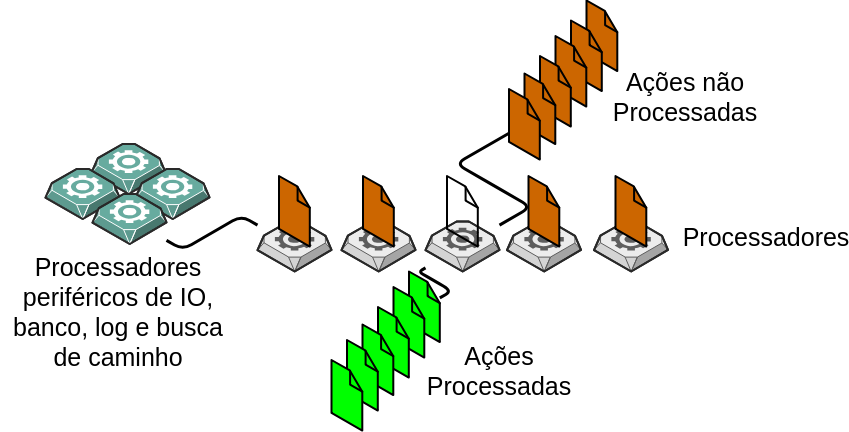
\includegraphics[height=6.5cm]{arquiteturas/salz_thread_model.png}
  \centering

  Adaptado de:~\cite{salz_albion, willson}.
\end{figure}



O microsserviço de jogo executa a lógica do jogo, visível na Figura~\ref{salz_thread_model}, para uma única área em um único processo.
%
Esta decisão é dada por conta da interação entre objetos ser complicada de executar em paralelo, visto o gerenciamento do custo de gerenciamento de semáforos necessários, caso execute estas ações em paralelo~\cite{salz_albion}.



Outra facilidade de implementar um modelo com um único processo para as interações entre objetos é facilitar o não manejo de objetos a qual não estão no campo de visão de todos os jogadores do serviço, realizando estas operações somente quando necessário~\cite{albion_online_unite, salz_albion}.


As entradas e saídas de mensagens(\textit{e.g.,} rede, Banco de dados, \textit{etc.}) e busca de caminho é executado por processos de trabalho separado do principal, utilizando a técnica de \textit{Thread Pool}~\cite{salz_albion, albion_online_unite, Ringler2014Dec}.
%
Todos os demais microsserviços operam sobre múltiplos processos, a partir do processo de conexão \ac{tcp} ao serviço~\cite{salz_albion}.
%
Diferente da arquitetura Rudy(Seção ~\ref{rudy}) a qual prioriza a resolução de requisições, evitando a executar métodos consecutivos da mesma conexão, na arquitetura Salz (Figura~\ref{full_salz}) as chamadas de processo remoto são executadas por ordem de chegada~\cite{salz_albion}.
%
Desta forma, quanto melhor a conexão com o serviço, mais requisições um cliente poderá executar.
%
Nesse sentido, uma conexão que transfere mais requisições terá mais vantagem sobre uma conexão a qual não transfere tantas requisições, executando mais operações por segundo.



Na arquitetura Salz, são necessárias três conexões \ac{tcp} com o servidor, de forma contínua~\cite{albion_online_unite}.
%
O custo desta operação é alto, e por isso nem sempre é viável utilizar esta abordagem, principalmente para jogos nos quais a demanda de banda seja menor.
%
Para evitar esta decisão, da mesma forma é notória a abordagem utilizada pela arquitetura Willson.



\subsection{Arquitetura elaborada por Willson}
\label{willson}


A arquitetura elaborada por Clarke-Willson leva como principal característica a preocupação da disponibilização de atualizações aos clientes~\cite{willson}.
%
Essas atualizações são versionadas a todos os microsserviços utilizando sistemas de versionamento de código fonte~\cite{stephenclarkewillson2017, willson}.
%
Por este motivo, a sua arquitetura inclusive compreende microsserviços de armazenamento de arquivos sobre protocolo \ac{http} para atualização dos clientes~\cite{stephenclarkewillson2017}.
%
Uma outra característica do serviço de jogo é a utilização de uma única conexão \ac{tcp} por cliente.
%
Essa arquitetura pode ser visualizada na Figura~\ref{full_willson}.


\begin{figure}[htb!]
  \caption{Arquitetura Willson.}
  \label{full_willson}
  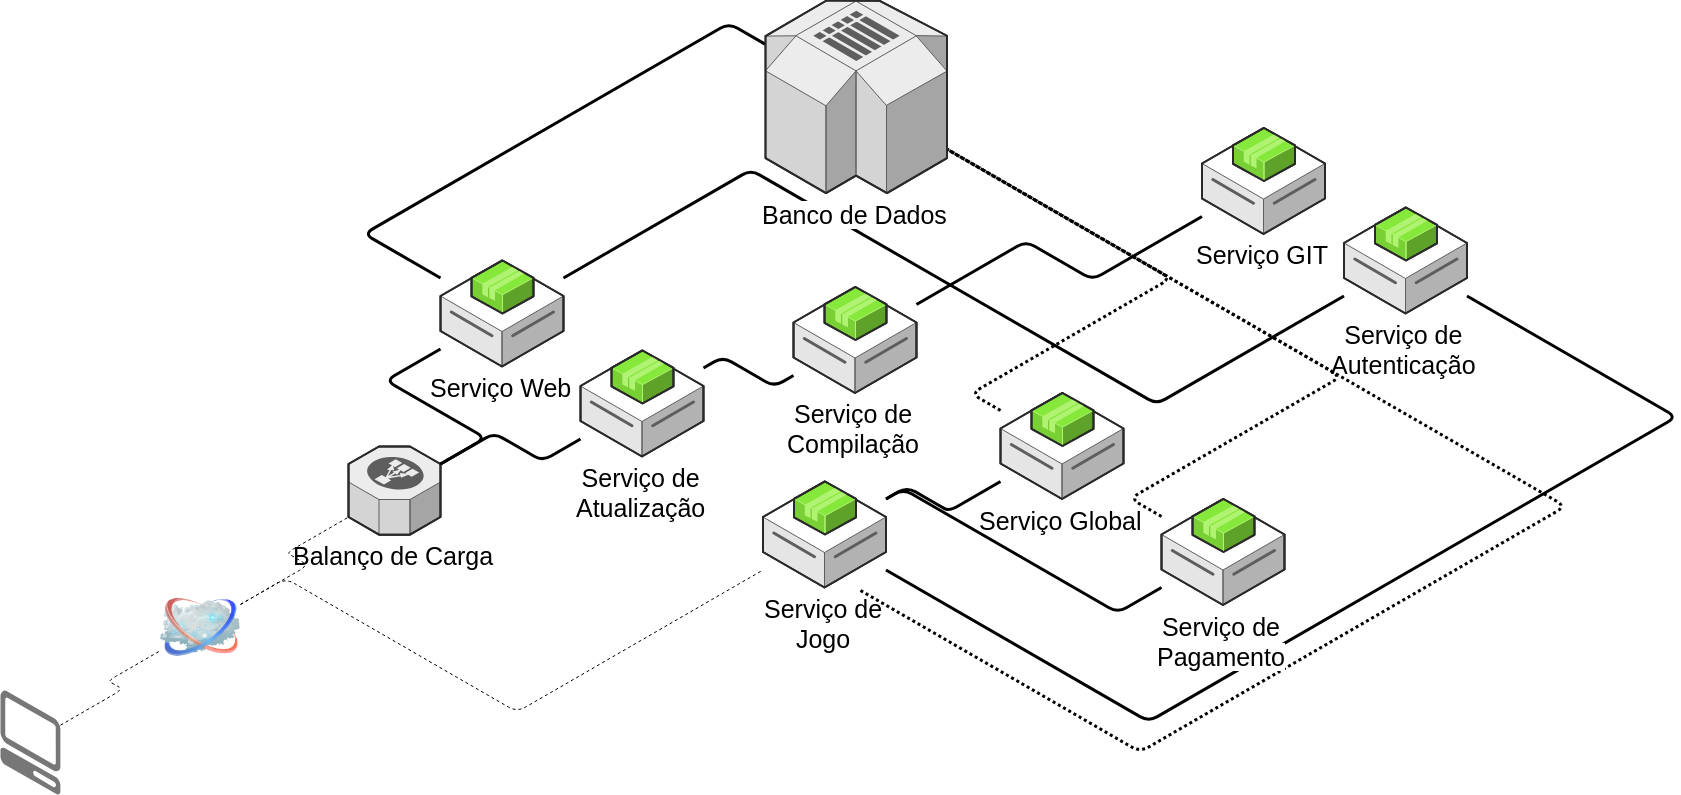
\includegraphics[width=\textwidth]{arquiteturas/full_willson.png}
  \centering

  Fonte:~\cite{stephenclarkewillson2017}.
\end{figure}


A arquitetura Willson, exibido na Figura~\ref{full_willson}, mostra um gradual entre a arquitetura Rudy (Figura~\ref{full_rudy}) e a arquitetura Salz (Figura~\ref{full_salz}), propondo uma arquitetura híbrida, na qual divide funcionalidades em outros microsserviços, porém ainda mantem diversas funcionalidade junto ao serviço de jogo evitando consumo de rede~\cite{albion_online_unite, willson}.
%
Essa abordagem garante menor latência de resposta, porém terá maior consumo de recursos da mesma máquina hospedeira do serviço~\cite{willson}.
%
Os microsserviços que compõem a arquitetura Willson são~\cite{willson, stephenclarkewillson2017}:

\begin{enumerate}
  \item \textbf{Serviço web}: Exibe informações do jogo, oferece operações \ac{crud} para cadastro de usuários e o sistema de pagamento. Opera sobre o protocolo \ac{http}.
  \item \textbf{Serviço de Atualização}: Integrado junto ao processo de desenvolvimento, fornecendo versionamento do cliente por um sistema web. Este microsserviço utiliza serviços internos ao desenvolvimento da aplicação. Opera sobre o protocolo \ac{http}.
  \item \textbf{Serviço de Autenticação e Social}: Gerencia a autenticação dos jogadores através de um serviço web. Também gerencia ações sociais (\textit{e.g.} sistema de amigos, grupos, nações, comércio, \textit{etc}). Opera sobre o protocolo \ac{http}.
  \item \textbf{Serviço de Balanceamento de carga}: Gerencia a carga entre os serviços web da arquitetura. Opera sobre o protocolo \ac{http}.
  \item \textbf{Serviço de Jogo}: Processa a lógica de jogo. Cada instância deste microsserviço gerencia um \textit{chunk} do ambiente do jogo. Opera sobre o protocolo \ac{rpc}.
  \item \textbf{Serviços Globais}: Processa rotinas globais do jogo, a qual não dependem do posicionamento do jogador. Opera sobre o serviço \ac{rpc}.
\end{enumerate}

O serviço de jogo da arquitetura Willson é comparada ao serviço similar na Salz~\ref{salz}, entretanto utiliza a técnica de \textit{thread pool} com valor de processos da fila de processadores fixo conforme o \textit{hardware} hospedeiro do serviço~\cite{stephenclarkewillson2017}.
%
Para modelos de paralelismo, pode-se utilizar os seguintes números processos paralelos~\cite{willson}:


\begin{enumerate}
  \item O dobro de número de núcleos: exige maior carga do serviço por troca de contexto entre os processos.
  \item O número exato de núcleos mais n: O serviço perderá tempo de processamento, trocando de contexto para outro processo, porém de forma mais sutil ao dobro do número de núcleos de processamento.
  \item O número de núcleos, exigindo um número menor de carga de contexto, dividindo somente com o sistema operacional.
  \item O número de núcleos menos um, liberando um núcleo para o sistema operacional.
\end{enumerate}

O número padrão de processos paralelos para processamento de requisições é o número de núcleos menos um, visando evitar a troca de contexto com o sistema operacional~\cite{willson}.
%
Essa troca de contexto trás variação na latência da resposta do serviço, a qual não tem controle pelo próprio serviço.
%
Nesse sentido, a melhor escolha é o número de núcleos menos um, escolhido após um teste de \textit{stress}~\ref{willson}.



Entretanto, não foi encontrado análises públicas sobre as arquiteturas Rudy, Salz e Willson, com relação ao uso de recursos dessas arquiteturas.
%
Nesse sentido, o atual trabalho define o seu problema sobre o consumo de recursos em buscar uma análise sobre o comportamento das arquiteturas referenciadas.

\section{Definição do Problema}



A escolha de uma arquitetura para serviços \ac{mmorpg} que não suportem uma elevada carga de trabalho podem ser um eventual problema na escalabilidade do negócio de empresas que forneçam tais serviços.
%
Em alguns serviços, a divisão da carga é dada pela área de interesse, dividindo o ambiente em pedaços a fim de diminuir a carga no serviço.
%
Porém, locais populares no ambiente do jogo ainda são vulneráveis a disponibilidade de serviço~\cite{1417630}.



Nesse sentido, arquiteturas de microsserviços surgiram com o objetivo de aumentar a disponibilidade e viabilizar produtos de demanda massiva.
%
Tais arquiteturas dividem o seu funcionamento em módulos menores a fim de proporcionar maior demanda utilizando uma abordagem distribuída.
%
Assim, o custo de atender uma alta demanda de conexões pode consumir uma quantia de recursos computacionais ou uma qualidade insatisfatória de serviço, inviabilizando a sua utilização no mercado.



Um exemplo de implementação de arquitetura de um jogo \ac{mmorpg} pode ser visualizado na Figura~\ref{fig:generica}, no qual cada cliente deve conectar em um microsserviço de gerenciamento de mundo para receber as atualizações da região e submeter seus comandos.
%
Nessa arquitetura, é necessário levar em conta o funcionamento, método de compartilhamento dos dados e abordagem para processamento do ambiente do jogo a fim de descrever a sua escalabilidade e qualidade de serviço.


\begin{figure}[htb!]
\caption{Arquitetura de um jogo \ac{mmorpg} genérico.}
\label{fig:generica}
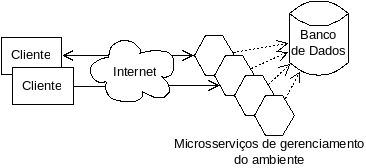
\includegraphics[height=9.0cm]{img/cap3/generica.png}
\centering

Fonte: O próprio autor
\end{figure}

A arquitetura genérica descrita na Figura~\ref{fig:generica} também precisa corresponder as demandas necessárias do \textit{GameDesign} do próprio jogo.
%
Neste caso, só um tipo de microsserviço é visível nesta rede, porém poderiam existir microsserviços responsáveis pela parte social, comércio e estatísticas, aumentando o grau de complexidade da arquitetura.
%
Em relação aos recursos utilizados por uma arquitetura, este trabalho foca na análise das arquiteturas de microsserviços descritas na literatura a fim de descrever o seu comportamento e desempenho.



A literatura aborda a previsibilidade de carga, análise de disponibilidade e uso de recurso de tais arquiteturas (a fim de guiar escolhas na etapa de \textit{Game Design} do produto e viabilizar o comércio do mesmo), relatados na Seção~\ref{sec:similares}.
%
Torna-se de interesse para empresas de desenvolvimento de jogos \ac{mmorpg} analisar o impacto e uso de recursos computacionais ao implantar uma arquitetura de microsserviços \ac{mmorpg} visando melhorar a disponibilidade de tais jogos.
%
Dentro do cenário de testes espera-se analisar por exemplo a estabilidade, limite de conexões e custo de processamento de tais arquiteturas.
%
Além disso, espera-se simular a carga de uma arquitetura utilizada em produção, a fim de possibilitar a quantificação do custo de operação de tal serviço.
%
Estas são expectativas gerais do que espera-se analisar, mas conforme a análise dos dados obtidos for realizada, é possível que outras características surjam.
%
Para guiar a proposta, um dos passos importantes são os trabalhos relacionados com este tema, na qual analisa-se estudos que abordam arquiteturas de jogos \ac{mmorpg} e/ou arquiteturas de microsserviços.



\section{Trabalhos Relacionados}
\label{sec:similares}



Para nortear o desenvolvimento da análise de microsserviços utilizados em jogos \ac{mmorpg} proposto no atual trabalho, essa seção apresenta outros trabalhos que têm o escopo ou objetivo similar, no qual monitoraram e analisaram serviços de jogos \ac{mmorpg} ou arquiteturas de microsserviços.
%
Ao apresentar estes trabalhos, busca-se apresentar o contexto e objetivo, e então aprofundar em características dos trabalhos, métricas utilizadas e ferramentas que auxiliaram nas análises.


Para encontrar os trabalhos relacionados, foi efetuada uma busca pelos termos \ac{mmorpg} ou \textit{microservices}.
%
Entretanto, os dois termos dificilmente se correlacionam nos meios de busca disponíveis para a elaboração deste TCC.
%
Nesse sentido, os trabalhos relacionados abordam arquiteturas de jogos \ac{mmorpg} ou arquiteturas de microsserviços.



Como critério de análise, foi observado em questão qual a classificação em que o trabalho encontra-se, entre previsão de carga ou análise de arquitetura, e quais métricas são utilizadas na análise.

\subsection{Huang et al. (2004)}
\label{sec:huang}



O trabalho de ~\cite{1417630} investiga a relação entre os recursos utilizados e o número de conexões presentes em um serviço \ac{mmorpg} distribuído.
%
Neste trabalho é relatado que a infraestrutura utiliza três serviços: Um \textit{Game Server} sobre protocolo \ac{tcp}, um \textit{Proxy Server} também sobre protocolo \ac{tcp}, e um servidor web para autenticação que executa sobre uma interface \ac{http}.
%
O foco de análise é o \textit{Proxy Server}, um serviço especificado em receber requisições e repassar atualizações da área de interesse destes jogadores, e o \textit{Game Server}, um serviço especificado para consumir as requisições realizadas pelo jogador.



\begin{figure}[htb!]
\caption{Arquitetura distribuída utilizando proxy.}
\label{fig:game_with_proxy}
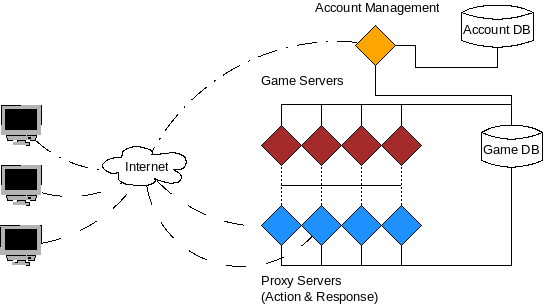
\includegraphics[width=\textwidth]{img/cap2/game_with_proxy.png}
\centering

Adaptado de:~\cite{1417630}.
\end{figure}



A infraestrutura do servidor de jogo contém um \textit{Proxy Server Farm} utilizando o algoritmo \textit{Round Robin} com pesos para balanceamento de carga entre cada cliente.
%
Cada \textit{Proxy Server} é responsável por comunicar com os demais microsserviços privados ao servidor, baseado com a área de interesse de sua conexão.
%
O protocolo de comunicação utilizado entre o Cliente e \textit{Proxy Server} é baseado em \ac{rpc}~\cite{faber, borella}, porém não é relatado sobre o o protocolo de comunicação utilizado entre o \textit{Proxy Server} e o \textit{Game Server}.
%
A sua arquitetura pode ser observada na Figura \ref{fig:game_with_proxy}, na qual obteve seus dados obtidos durante 100 dias para realizar as análises.
%
A Figura \ref{fig:players_peer_time} demonstra uma amostra do número de conexões pelo tempo no serviço obtido.



\begin{figure}[htb!]
\caption{Número de conexões no serviço pelo tempo decorrido.}
\label{fig:players_peer_time}
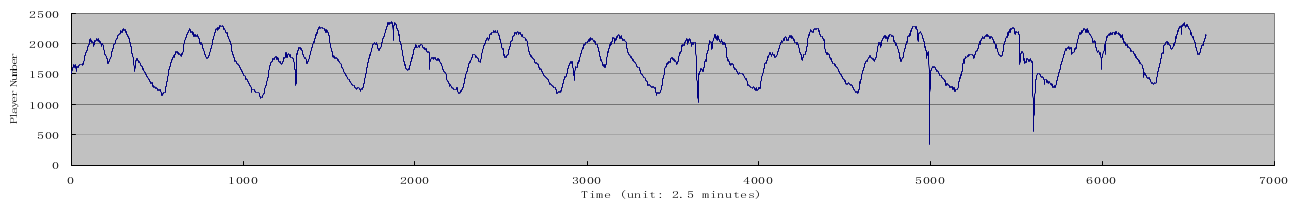
\includegraphics[width=\textwidth]{img/cap2/players_peer_time.png}
\centering

Fonte:~\cite{1417630}.
\end{figure}



Como análise, o autor correlacionou o número de conexões com número de pacotes e banda, consumidos, utilizando uma função estatística linear.
%
Esta função pode ser utilizada com regressão linear para prever consumo de recursos futuros e por fim realocar mais recursos ao serviço, contribuindo com escalabilidade vertical autônoma.
%
Um exemplo de aplicação dessa regressão linear pode ser visualizada na Figura~\ref{fig:regressao_bytes}, no qual o autor compara o consumo de banda real comparado a regressão linear.



\begin{figure}[htb!]
\caption{Regressão linear comparado ao consumo de banda real do servidor.}
\label{fig:regressao_bytes}
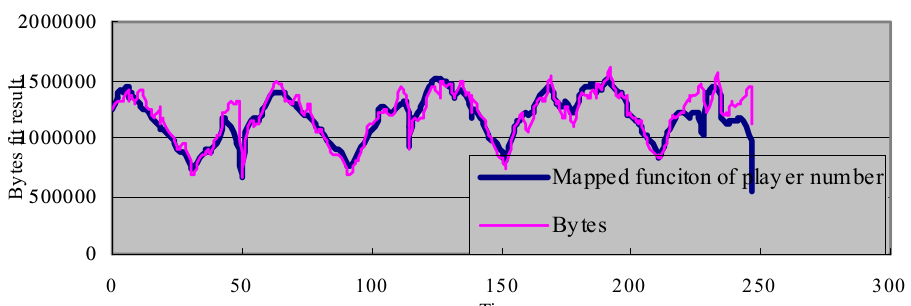
\includegraphics[width=\textwidth]{img/cap2/regressao.png}
\centering

Fonte:~\cite{1417630}
\end{figure}



Entretanto, a escalabilidade horizontal não pode ser prevista, visto que não é analisado o posicionamento de cada personagem a fim de dividir os ambientes em pedaços menores com outros serviços.
%
Como trabalhos futuros é relatado a análise do posicionamento de personagens para escalabilidade horizontal, a análise de outras arquiteturas e a análise de outros gêneros de jogos, além do impacto de utilizar balanço de carga e provisionamento de recursos de forma dinâmica.



\subsection{Villamizar et al. (2016)}



O trabalho de ~\cite{7515686} investiga o custo de arquiteturas de microsserviços, arquiteturas \ac{paas} orientadas a eventos e aplicações monolíticas para aplicações web.
%
A sua principal motivação é a comparação de custos para a tradução de sistemas legados para arquiteturas distribuídas.
%
Para isso, o autor preparou três instâncias de testes com suas configurações desenhadas a fim de ter o maior número de requisições por minuto com o mesmo custo financeiro.



\begin{figure}[htb!]
\caption{Arquitetura monolítica web implementada na \ac{aws}.}
\label{fig:aws_monolitico}
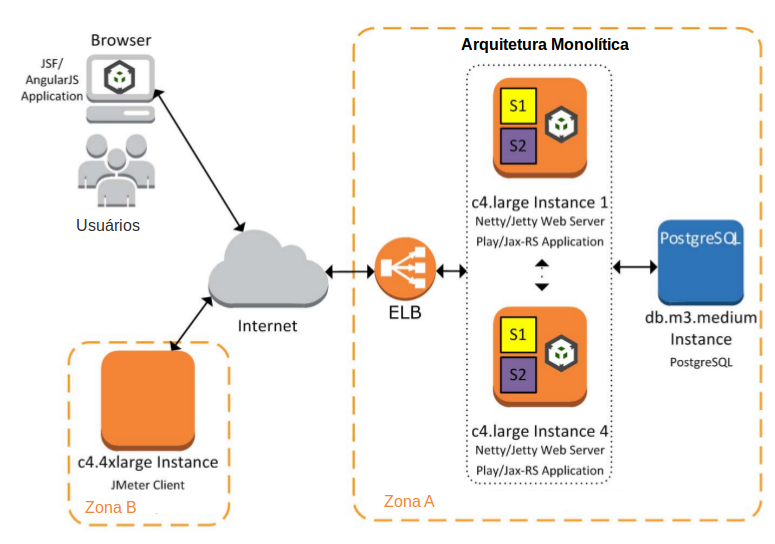
\includegraphics[width=\textwidth]{img/cap2/aws_monolitico.png}
\centering

Fonte:~\cite{7515686}
\end{figure}


\textbf{Instância I.} Utilizando quatro instâncias \ac{aws} \textit{c4.large}, uma instância \ac{aws} \textit{c4.xlarge} e uma instância \ac{aws} \textit{db.m3.medium}.
%
A Figura~\ref{fig:aws_monolitico} exibe a implantação de uma aplicação web monolítica.
%
Essa arquitetura foi implementada utilizando \textit{Jax-RS} e \textit{Play Framework}.




\begin{figure}[htb!]
\caption{Arquitetura de microsserviços web implementada na \ac{aws}.}
\label{fig:aws_microsservicos}
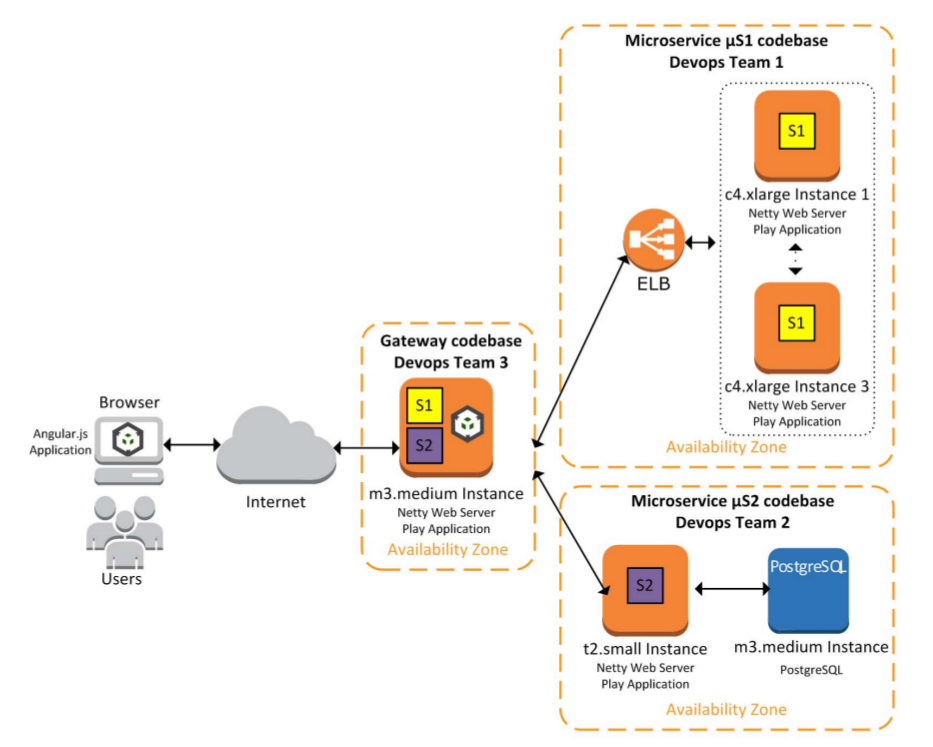
\includegraphics[width=\textwidth]{img/cap2/aws_microsservicos.png}
\centering

Fonte:~\cite{7515686}
\end{figure}

\textbf{Instância II.} Utilizando três instâncias \ac{aws} \textit{c4.xlarge}, uma instância \ac{aws} \textit{t2.small} e uma instância \ac{aws} \textit{db.m3.medium}.
%
A Figura~\ref{fig:aws_microsservicos} exibe a implantação de uma aplicação de microsserviços web. Essa arquitetura foi implementada utilizando \textit{Play Framework}, framework para desenvolvimento web para a linguagem Java e Scala~\footnote{Play Framework: \url{https://www.playframework.com/}}.



\begin{figure}[htb!]
\caption{Arquitetura de microsserviços web implementada na \ac{aws} utilizando a tecnologia \textit{lambda}.}
\label{fig:aws_lambda}
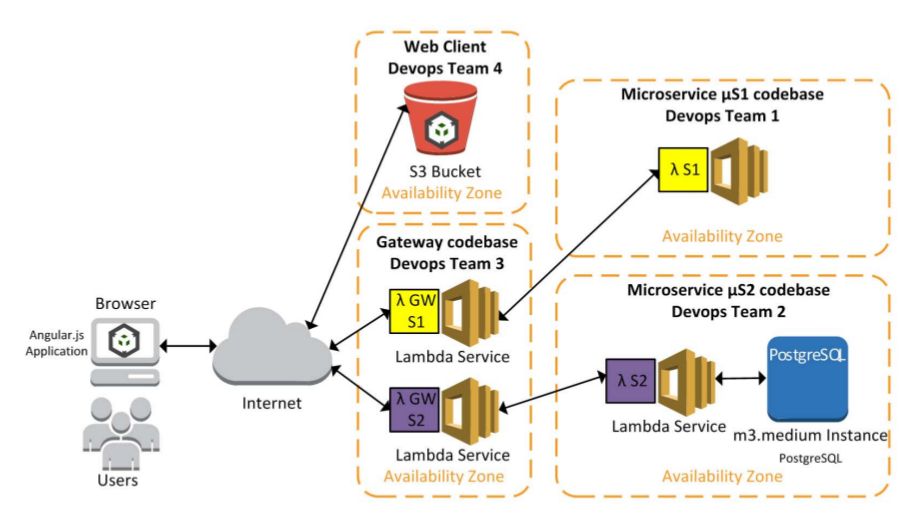
\includegraphics[width=\textwidth]{img/cap2/aws_lambda.png}
\centering

Fonte:~\cite{7515686}
\end{figure}

\textbf{Instância III.} Utilizando duas instâncias \ac{aws} \textit{lambda S1}, duas instâncias \ac{aws} \textit{lambda S2}, uma instância \ac{aws} \textit{S3 Bucket} e uma instância \ac{aws} \textit{db.m3.medium}.
%
A Figura~\ref{fig:aws_lambda} exibe a implantação de uma aplicação de microsserviços web utilizando a tecnologia \ac{aws} \textit{lambda}. Essa arquitetura foi implementada utilizando o \textit{framework} \textit{Node.js}\footnote{Node.js: \url{https://nodejs.org/en/}}, nas quais as funções de \textit{gateway} são implementadas em quatro funções independentes do tipo \textit{microservice-http-endpoint}.



\begin{figure}[htb!]
\caption{Custo por um milhão de requisições em dólares utilizando diferentes arquiteturas sobre a \ac{aws}.}
\label{fig:custo_aws}
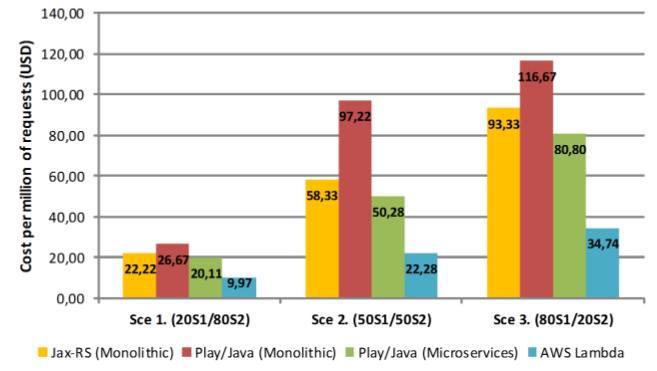
\includegraphics[width=\textwidth]{img/cap2/custo_aws.png}
\centering

Fonte:~\cite{7515686}
\end{figure}



Foi concluído que a arquitetura de microsserviços, nas condições desta aplicação, podem reduzir até 13.42\% em gastos com a infraestrutura.
%
Essa redução pode ser observada na Figura~\ref{fig:custo_aws}.
%
O autor alerta sobre tolerância a falhas, transações distribuídas, distribuição de dados e versionamento de serviço.


\subsection{Suznjevic e Matijasevic (2012)}



O trabalho de ~\cite{6374456} tem seu objetivo a fim de prever a carga a qual um serviço \ac{mmorpg} pode receber utilizando a complexidade das operações nos contextos de \ac{pvp} e \ac{pvnpc} a qual um personagem pode realizar em um ambiente.
%
Este trabalho usa com base o modelo descrito na Seção~\ref{sec:huang}, um modelo distribuído em serviços na qual efetuam o processamento de uma região do ambiente virtual.



\begin{table}[htb!]
\centering
\caption{Complexidade da interação com o ambiente, por contexto da interação.}
\label{tab:complexidade}
\begin{tabular}{|l|l|l|l|l|}
\hline
Contexto da ação        & \ac{pvp}           & \ac{pvnpc}              & Número de \acp{npc}    & Network {[}kbits/s{]} \\ \hline
Questing                & $O(n)$             & $O(n log(n))$           & $N \leq 6 $            & 11.4          \\ \hline
Trading                 & $O(n)$             & $O(n)$                  & $N \leq 20$            & 8.1           \\ \hline
Dungeons                & $O(n^2)$           & $O(n^2)$                & $N \leq 20$            & 18.3          \\ \hline
\ac{pvp} combat         & $O(n^3)$           & $O(n)$                  & $N = 0    $            & 24.1          \\ \hline
Raiding                 & $O(n^2 log(n))$    & $O(n^3)$                & $N \leq 40$            & 32.0          \\ \hline
\end{tabular}

Fonte:~\cite{6374456}
\end{table}


A análise realizada leva em conta a complexidade das ações no ambiente, a qual pode ser descrita na Tabela~\ref{tab:complexidade}.
%
Essa tabela exibe as ações que podem ser executadas para interagir com o ambiente, seja essa interação com \ac{pvp} (jogador com outro jogador) ou \ac{pvnpc} (jogador com um personagem ou objeto gerenciado pelo serviço).
%
Os contextos analisados nessa tabela são:

\begin{itemize}
  \item \textit{Questing}: Contexto de missão, na qual um grupo de jogadores ou um grupo de \acp{npc} podem ser afetados nas ações.
  \item \textit{Trading}: Contexto de negociação, na qual a complexidade leva em conta somente o número de itens negociados.
  \item \textit{Dungeons}: Contexto de exploração, na qual o ambiente pode ser modificado conforme as ações dos personagens em um ambiente isolado para este grupo.
  \item \textit{\ac{pvp} combat}: Contexto de batalha entre jogadores, na qual as ações entre os jogadores influenciam diretamente o estado do personagem oponente.
  \item \textit{Raiding}: Representa um contexto específico de exploração, na qual múltiplos jogadores unem forças a fim de combater outro grupo de jogadores ou \acp{npc}.
\end{itemize}


\begin{figure}[htb!]
\caption{Regressão levando em conta a complexidade das ações e contexto dos personagens.}
\label{fig:regressao_complexidade}
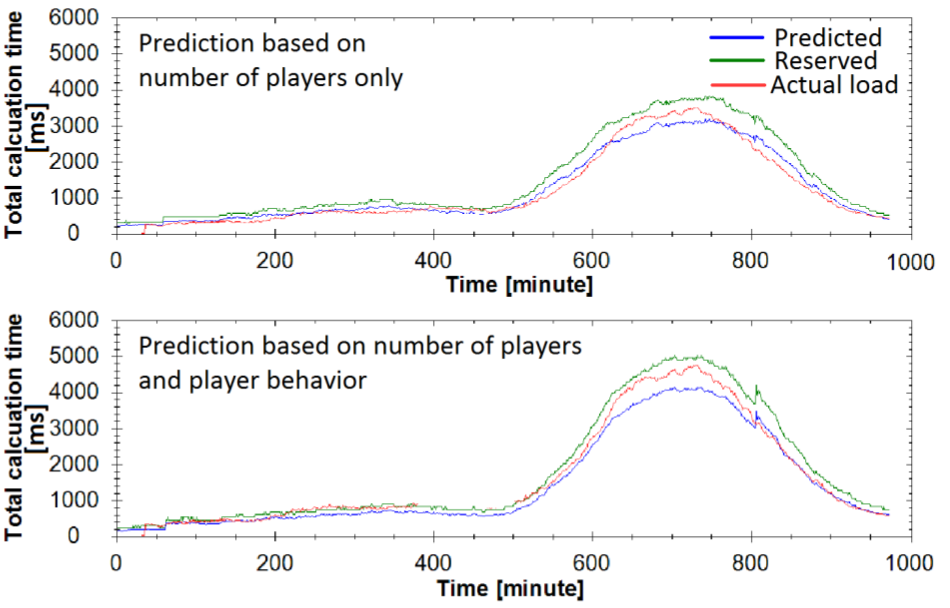
\includegraphics[width=\textwidth]{img/cap2/network_regressao_complexidade.png}
\centering

Fonte:~\cite{6374456}
\end{figure}


Utilizando as complexidades das ações, o número de conexões e o contexto de cada personagem no ambiente para predizer a banda utilizada.
%
Pode-se visualizar uma regressão na Figura~\ref{fig:regressao_complexidade}.



O autor conclui que o contexto de interação com o ambiente de cada personagem tem relevância com o consumo de \ac{cpu} e banda, a qual pode ser calculada com sua complexidade a fim de desenvolver uma ferramenta para predição de carga sobre serviços \ac{mmorpg}.
%
Entretanto, essa predição não é feita em tempo real, não contribuindo para a automação da escalabilidade vertical e horizontal da arquitetura de microsserviços.



\subsection{Análise dos trabalhos relacionados}
\label{sec:similares_analise}



Para os trabalhos relacionados, são analisados o tipo de pesquisa realizado sobre Microsserviços e serviços \ac{mmorpg}.
%
Também são levantados quais os recursos computacionais relacionados com estas análises.


Nos trabalhos relacionados existem duas abordagens utilizadas pelos autores, na qual estão relacionados a Previsão de Carga ou Comparação entre Arquiteturas de microsserviços~\cite{7515686, 6374456}:

\begin{itemize}
  \item \textbf{Comparação de arquiteturas}: O autor utiliza alguma métrica a fim de decidir qual a melhor alternativa de arquitetura para determinada aplicação.
  \item \textbf{Previsão de carga}: Projetar a carga futura sobre algum recurso a fim de escalar automaticamente a sua arquitetura na nuvem, a fim de reduzir gastos de recursos ociosos e diminuir o impacto de ocorrências aos usuários finais.
\end{itemize}

Dessa forma, pode-se dividir os trabalhos relacionados com a sua categoria.
%
Esta relação pode ser visualizada na Tabela~\ref{tab:categoria_trabalhos}.

\begin{table}[htb!]
\centering
\caption{Trabalhos relacionados por categoria.}
\label{tab:categoria_trabalhos}
\begin{tabular}{l|l}
\hline
Autor & Categoria                            \\ \hline
\cite{6374456}  & Previsão de carga          \\ \hline
\cite{7515686}  & Comparação de arquiteturas \\ \hline
\cite{1417630}  & Previsão de carga          \\ \hline
\end{tabular}


Fonte: O próprio autor.
\end{table}

Para o trabalho referente a comparação de arquiteturas~\cite{7515686}, o recurso utilizado foi o custo por um determinado número de requisições web.
%
Já para os trabalhos referentes a previsão de carga~\cite{6374456, 1417630} foi levantado o consumo da banda, \ac{cpu} e memória, entretanto não levantou-se o número de conexões e latência aos usuários, na qual podem ser observados na Tabela~\ref{tab:recursos_categoria}.
%
Nenhum trabalho relatou limite de conexões ou latência do sistema.

\begin{table}[htb!]
\centering
\begin{adjustbox}{max width=\textwidth}
\caption{Trabalhos relacionados por recurso analisado.}
\label{tab:recursos_categoria}
\begin{tabular}{l|l|l|l|l|l|l|l}
\hline
Autor           & \ac{cpu}   & Memória    & Banda      & Custo      & Latência & \makecell{Limite \\ de \\ conexões} & \makecell{Complexidade \\ de \\ Algoritmos} \\ \hline
\cite{1417630}  & $\times$   & $\times$   & \checkmark & $\times$   & $\times$ & $\times$                            & $\times$                                    \\ \hline
\cite{7515686}  & $\times$   & $\times$   & $\times$   & \checkmark & $\times$ & $\times$                            & $\times$                                    \\ \hline
\cite{6374456}  & \checkmark & \checkmark & \checkmark & $\times$   & $\times$ & $\times$                            & \checkmark                                  \\ \hline
\end{tabular}
\end{adjustbox}

Fonte: O próprio autor.
\end{table}



Outro ponto a ser analisado são as arquiteturas utilizadas. Os trabalhos referentes a previsão de carga não utilizaram uma arquitetura de microsserviços, mesmo sendo um sistema distribuído.
%
Nesses serviços, os sistemas eram dependentes entre sí e precisavam um dos outros para o seu funcionamento.
%
A relação de arquiteturas abordadas pode ser visualizado na Tabela~\ref{tab:arquiteturas_analisadas}, na qual mostra quais trabalhos abordaram os temas sobre arquiteturas de microsserviços e jogos \ac{mmorpg}.
%
Além disso, não foi descrito um método de replicação automática dos serviços a fim de prover alta disponibilidade de forma automatizada, sendo abordado como um trabalho futuro.


\begin{table}[htb!]
\centering
\begin{adjustbox}{max width=\textwidth}
\caption{Arquiteturas analisadas.}
\label{tab:arquiteturas_analisadas}
\begin{tabular}{l|l|l|l}
\hline
Autor           & Arquitetura de Microsserviços & Arquitetura Distribuída  & \ac{mmorpg}   \\ \hline
\cite{1417630}  & $\times$                      & \checkmark               & \checkmark    \\ \hline
\cite{7515686}  & \checkmark                    & \checkmark               & $\times$      \\ \hline
\cite{6374456}  & $\times$                      & \checkmark               & \checkmark    \\ \hline
\end{tabular}
\end{adjustbox}

Fonte: O próprio autor.
\end{table}


Este Trabalho de Conclusão de Curso pretende analisar uma arquitetura de microsserviços especificada a jogos \ac{mmorpg}, visando métricas de desempenho e custo de operação.
%
Os recursos analisados serão CPU, Memória, Banda, Custo, Latência, Limite de Conexões e Complexidade dos Algoritmos empregados.


\section{Considerações parciais}

Este capítulo conceituou jogos eletrônicos, gênero de jogo e especificou as características de um jogo \ac{mmorpg}.
%
Após apresentar sobre o gênero de jogo abordado, detalha-se a sua jogabilidade, problemas relevantes a este gênero do ponto de vista de rede de computadores e por fim sobre técnicas e abordagens populares acerca do desenvolvimento destes serviços, a qual serão utilizados no problema deste Trabalho de Conclusão de Curso.


Por fim, são apresentados trabalhos relacionados a fim de guiar por métricas, métodos de coleta de dados e métodos de desenvolvimento e implantação de tais arquiteturas a fim de contribuir com o atual escopo do trabalho.
%
Entretanto, houve uma dificuldade em encontrar na literatura análises sobre arquiteturas de microsserviços focado a jogos, principalmente em específico o gênero \ac{mmorpg}.
%
Dessa forma, espera-se introduzir a analise da viabilidade e do custo de recursos computacionais para manter um serviço \ac{mmorpg} sobre uma arquitetura de microsserviços.
